%% This is a skeleton file to create IEEE style Bibliography list. There is a guide added "create-manual-bib-entry.txt" to manually create popular types of references such as PhD thesis, website, unpublished work etc.
%%
%% Modified by K. Reaz( kahn.reaz@ieee.org)
%% Support sites:
%% http://www.ieee.org/

%%***********************************************************
%% Legal Notice:
%% This code is offered as-is without any warranty either expressed or implied; without even the implied warranty of MERCHANTABILITY or FITNESS FOR A PARTICULAR PURPOSE! 
%% User assumes all risk and can modify as s/he wants.

%%***********************************************************

%package list
\documentclass[conference]{IEEEtran}
\usepackage{cite}
\usepackage{cite}
\usepackage{amsmath,amssymb,amsfonts}
\usepackage{algorithmic}
\usepackage{graphicx}
\usepackage{textcomp}
\usepackage{xcolor}
\usepackage{dirtytalk}
\usepackage{csquotes}
\usepackage[export]{adjustbox}
\usepackage[pdftex]{graphicx}

\def\BibTeX{{\rm B\kern-.05em{\sc i\kern-.025em b}\kern-.08em
    T\kern-.1667em\lower.7ex\hbox{E}\kern-.125emX}}
\author{Ali Al Shami$^{1}$}

\thanks{Ali Al Shami with the Computer Science Department, University of Colorado Colorado Springs, Colorado Springs, CO, 80918 USA e-mail:(aalshami@uccs.edu)}
\begin{document}
%Here goes the title
\title{Journal 1}
\maketitle

%Main body starts
\section{Introduction}
I am Ali Alshami, a Ph.D. student in computer science and a Graduate Research Assistant (GRA) at the Vision Security Technology (VAST) Lab, the University of Colorado Colorado Springs (UCCS).

My goal for the course is to finish and submit a survey paper on human action recognition and prediction and start a new paper that focuses on predicting the future movement of humans based on human pose estimation and motion information. The survey paper reviews and evaluates the recent human actions recognition and prediction papers based on vision and machine learning. The new work will be focused on predicting the future movement of humans in video based on past movement, motion information, and human pose estimation.

I hope to learn more about improving my research skills and what I must consider becoming a better researcher. I am also curious about how to convert research that we are working on to a product you and what things we need to consider to make it a successful product.

I enjoy outdoor activities, including running, hiking, mountain biking, tennis, pickle-ball, and snowboarding. I also like reading and playing piano sometimes.
\begin{figure}[hbt!]
    \centering
    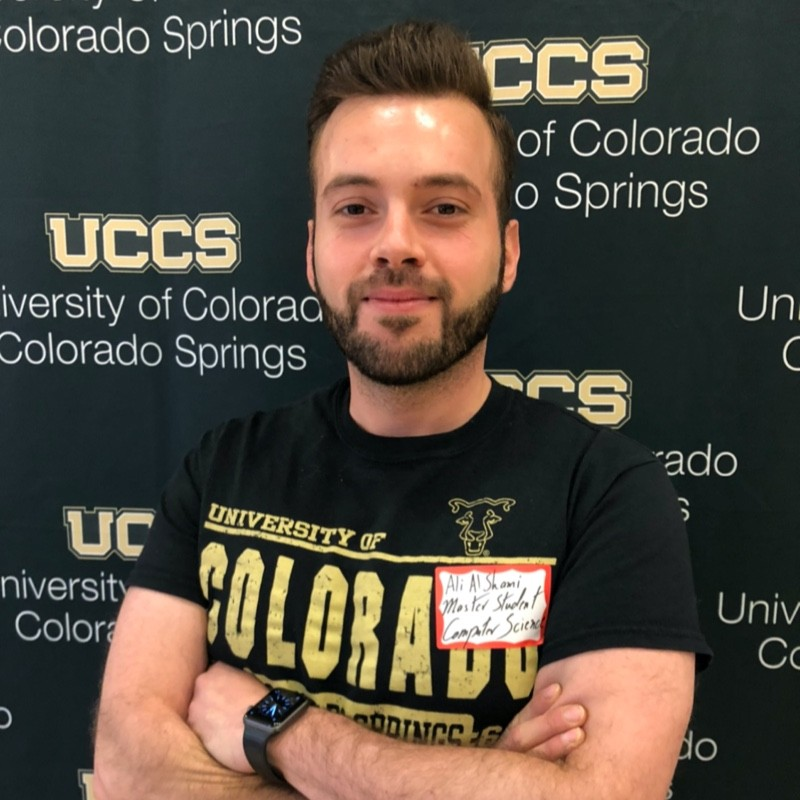
\includegraphics[width=5cm]{alshami.jpg}
    \caption{ }
    \label{fig:Remove}
\end{figure}
\section{Ask question here}
If you dont mind me asking what was your masters and bachelors in because Im curious on what led to that specific topic of research? If its the same as your Ph.D. then what did lead to you becoming intrested in your area of research? -Noah Rodgers

\bibliographystyle{IEEEtran}
\bibliography{main}

\end{document}
